\chapter{Results}
\label{ch:results}

This chapter presents the results of our model training and evaluation. We tested Decision Tree, K-Nearest Neighbors (KNN), and Random Forest regressors to predict next-year home value growth using a ZIP-based test split. The following sections show how model performance varies with feature selection, test accuracy, and behavior over time.

\section{Feature selection and model comparison}

We used mutual information and f-regression to rank features, then evaluated model performance using the top-$k$ features for $k \in [1, 50]$. Figures below show the 3-fold cross-validated $R^2$ scores across feature counts.

\begin{figure}[!ht]
    \centering
    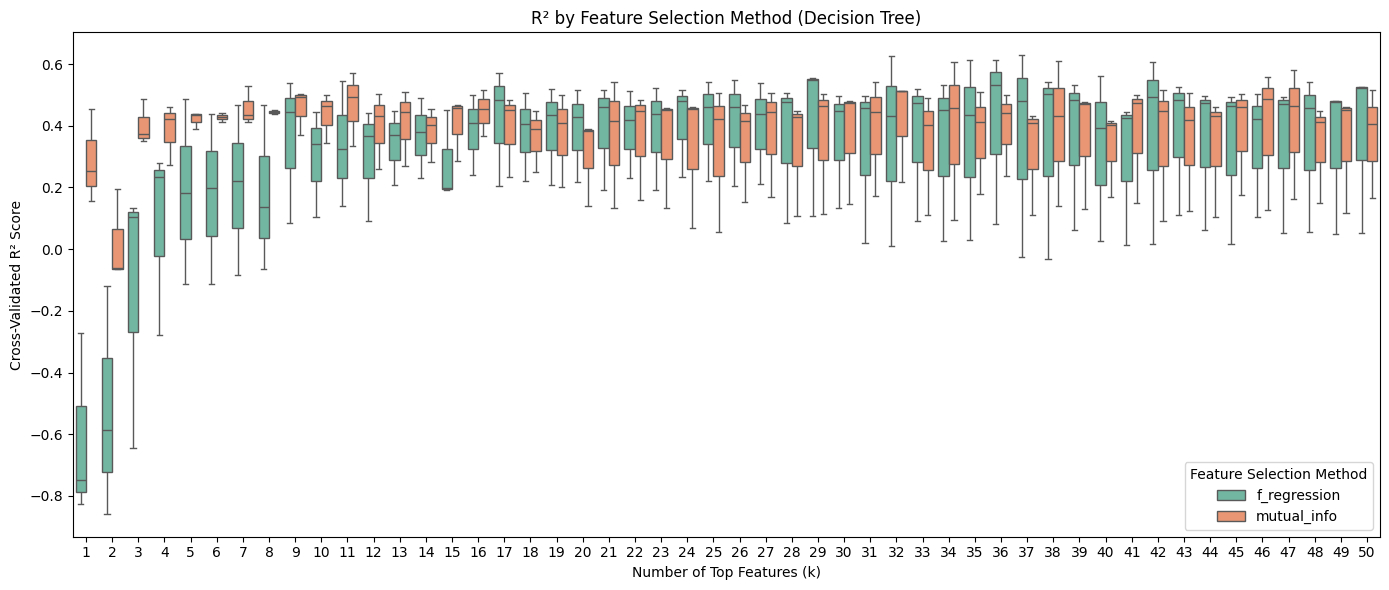
\includegraphics[width=\textwidth]{figures/box50_DT.png}
    \caption{Feature selection performance for Decision Tree}
    \caption*{\hspace{1em}}
    \label{fig:box_dt}
\end{figure}
\FloatBarrier

Decision Tree improves up to about 8–10 features, then rapidly declines. This is especially evident when using mutual information, which adds non-linear but noisy variables. The model is sensitive to irrelevant input and prone to overfitting.

\begin{figure}[!ht]
    \centering
    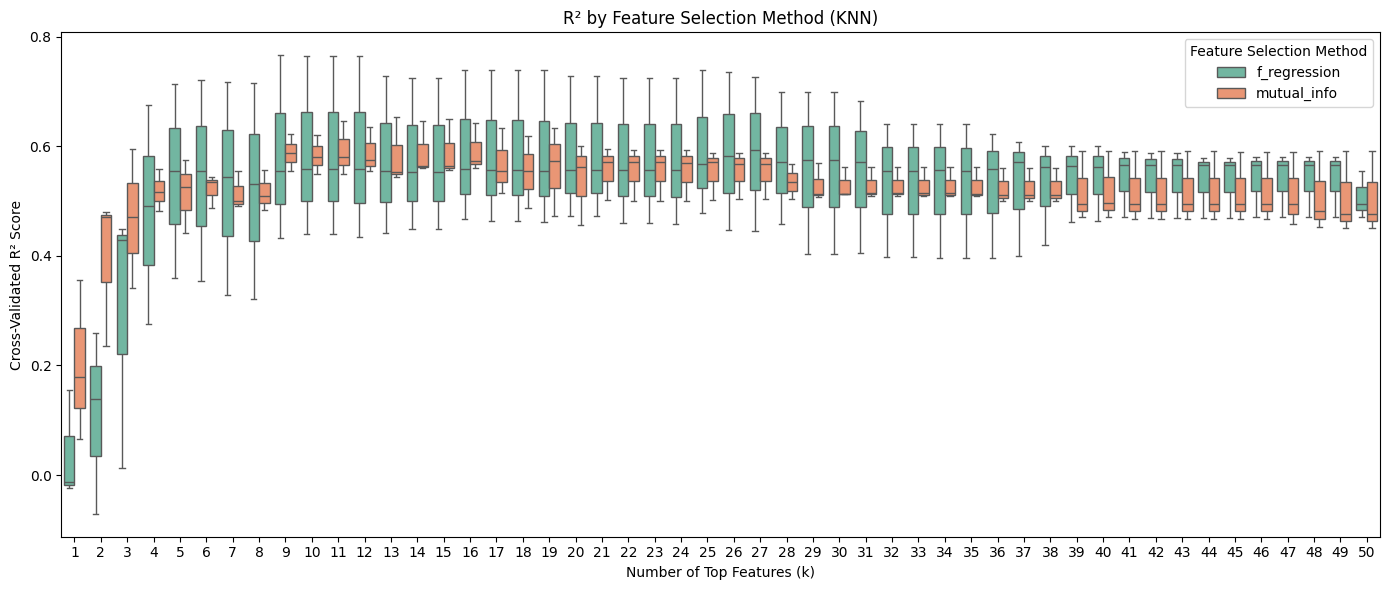
\includegraphics[width=\textwidth]{figures/box50_KNN.png}
    \caption{Feature selection performance for K-Nearest Neighbors}
    \caption*{\hspace{1em}}
    \label{fig:box_knn}
\end{figure}
\FloatBarrier

KNN performance increases up to 9 features, then plateaus. f-regression works best at low $k$, while mutual information stabilizes later. This shows that KNN benefits from smaller, more targeted feature sets and becomes unstable with excess input.

\begin{figure}[!ht]
    \centering
    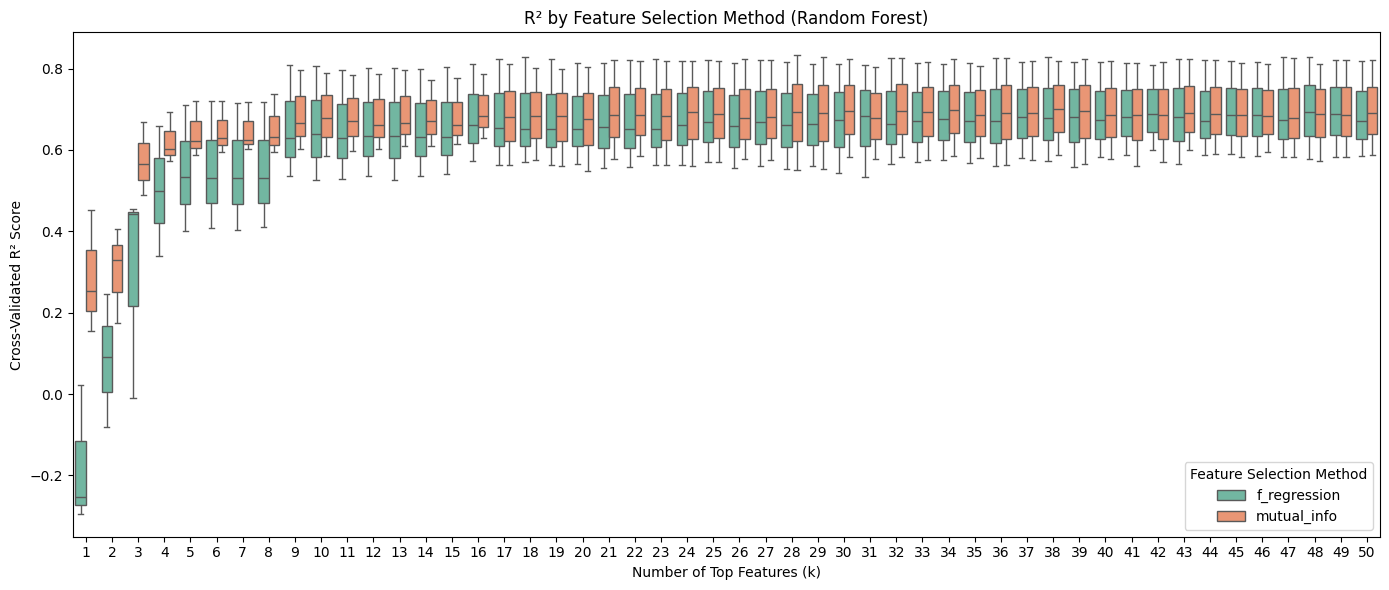
\includegraphics[width=\textwidth]{figures/box50_RF.png}
    \caption{Feature selection performance for Random Forest}
    \caption*{\hspace{1em}}
    \label{fig:box_rf}
\end{figure}
\FloatBarrier

Random Forest improves steadily up to about 16 features and holds steady beyond that. Its low variance and tolerance for redundant input reflect the model’s robustness and internal feature selection behavior.

\section{Model prediction performance}

This section evaluates how well each model predicts on unseen ZIP codes. For each model, we compare test set accuracy and generalization behavior by plotting predicted vs actual YoY values and train vs test predictions.

\subsection{Decision Tree}

\begin{figure}[!ht]
    \centering
    \subfigure[]{%
        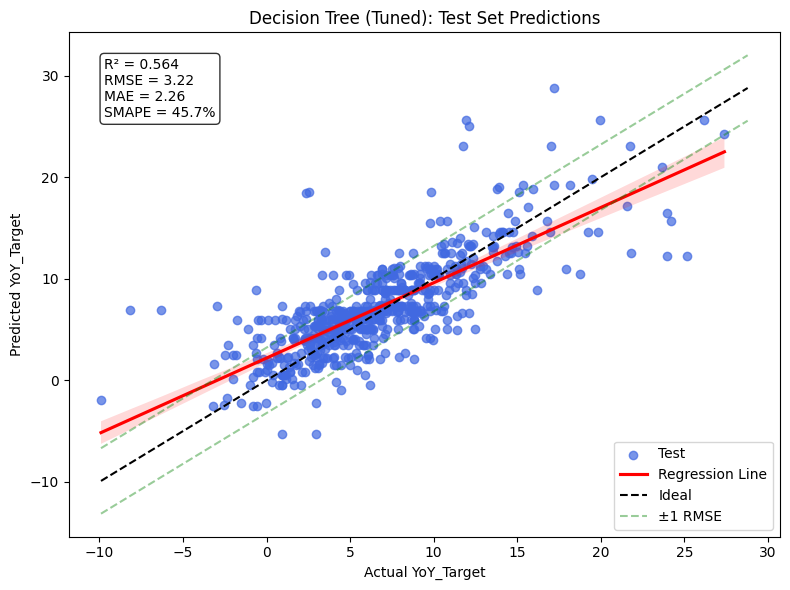
\includegraphics[width=0.48\textwidth]{figures/DT1.png}
    }\hfill
    \subfigure[]{%
        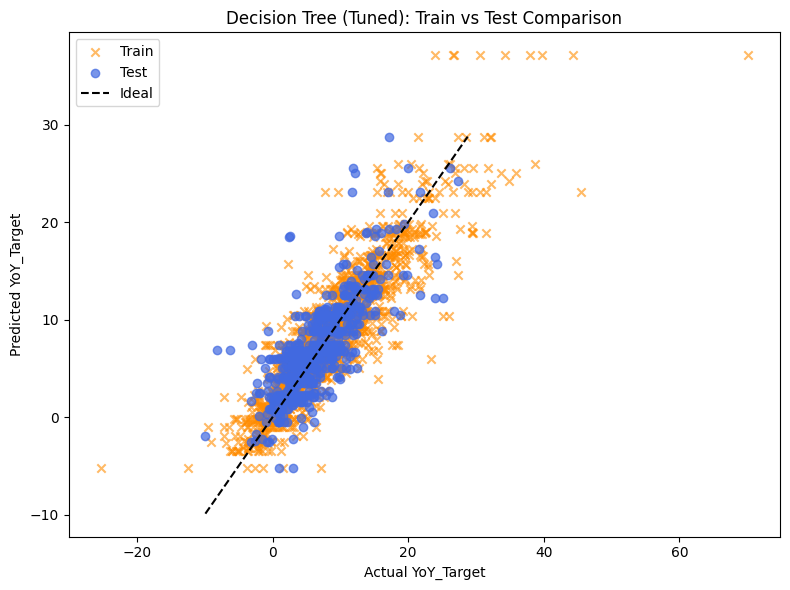
\includegraphics[width=0.48\textwidth]{figures/DT2.png}
    }
    \caption{Decision Tree test performance}
    \caption*{\hspace{1em}}
    \label{fig:dt_results}
\end{figure}
\FloatBarrier

The Decision Tree model underperforms relative to the other models. In Figure~\ref{fig:dt_results}a, test predictions are concentrated near the mean, failing to capture the spread in actual values. The regression line is shallow and diverges significantly from the ideal diagonal. Figure~\ref{fig:dt_results}b shows that while the model fits the training set tightly, it generalizes poorly. This indicates overfitting, which is consistent with its lower $R^2$ score and wider error margins on the test set.

\subsection{K-Nearest Neighbors (KNN)}

\begin{figure}[!ht]
    \centering
    \subfigure[]{%
        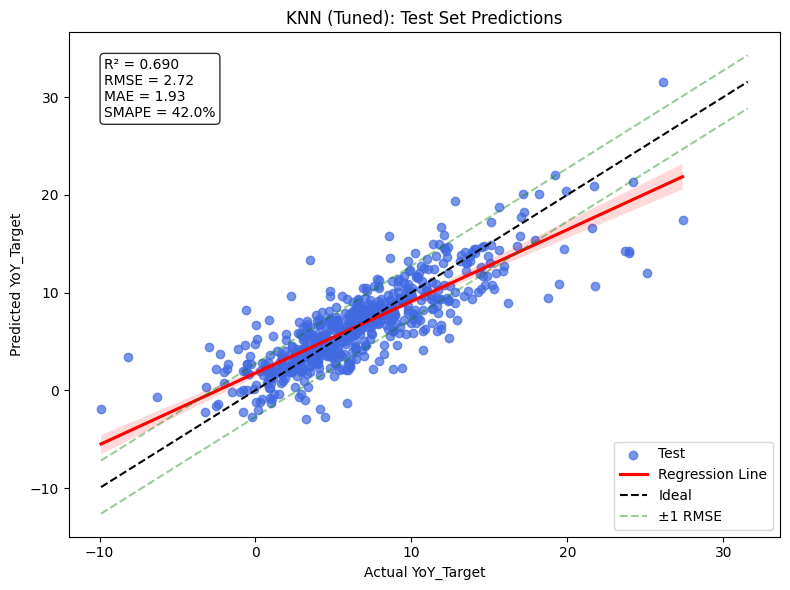
\includegraphics[width=0.48\textwidth]{figures/KNN1.png}
    }\hfill
    \subfigure[]{%
        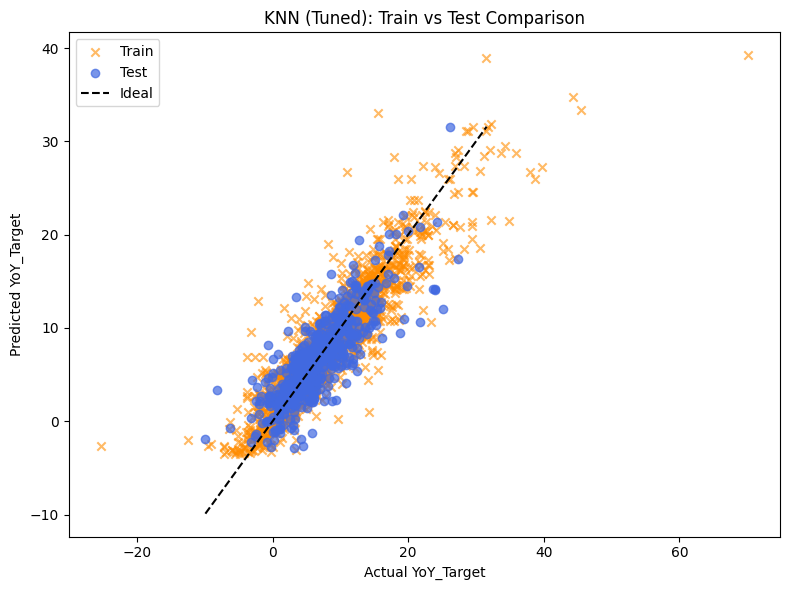
\includegraphics[width=0.48\textwidth]{figures/KNN2.png}
    }
    \caption{KNN test performance}
    \caption*{\hspace{1em}}
    \label{fig:knn_results}
\end{figure}
\FloatBarrier

Figure~\ref{fig:knn_results}a shows that KNN predictions align more closely with actual values compared to Decision Tree, especially in the mid-range. However, the model tends to underpredict at the higher end of the target range. In Figure~\ref{fig:knn_results}b, training predictions are tighter than the test predictions, which show more scatter. This reflects the model’s reliance on similar training examples; when ZIPs with comparable patterns exist in the training data, KNN performs well, but it generalizes less effectively for outlier regions.

\subsection{Random Forest}

\begin{figure}[!ht]
    \centering
    \subfigure[]{%
        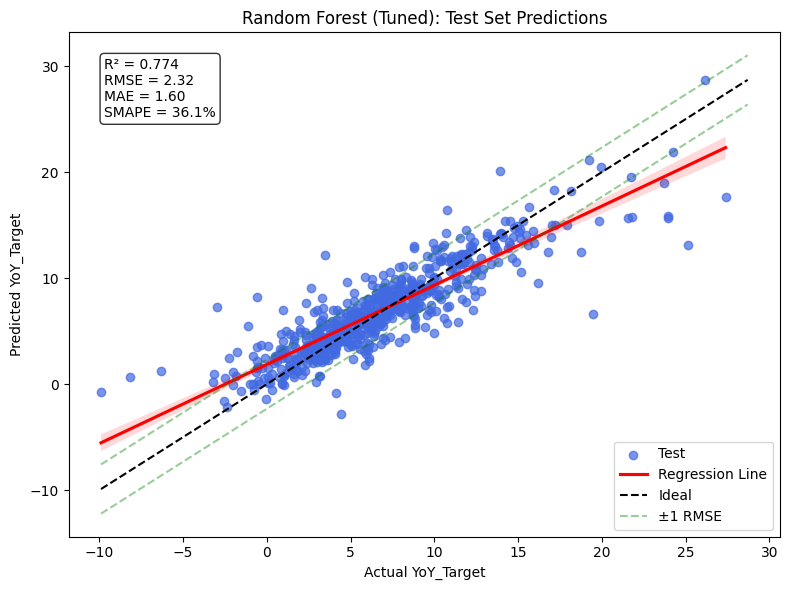
\includegraphics[width=0.48\textwidth]{figures/RF1.png}
    }\hfill
    \subfigure[]{%
        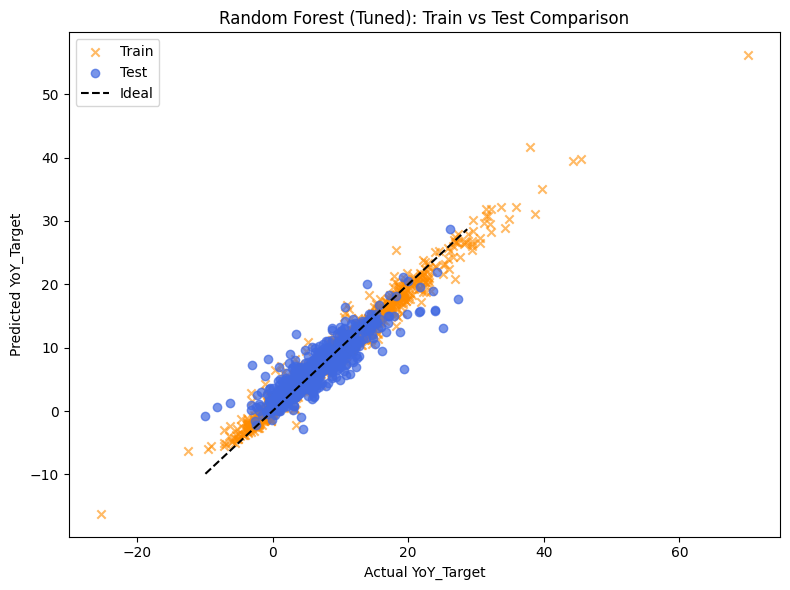
\includegraphics[width=0.48\textwidth]{figures/RF2.png}
    }
    \caption{Random Forest test performance}
    \caption*{\hspace{1em}}
    \label{fig:rf_results}
\end{figure}
\FloatBarrier

Figure~\ref{fig:rf_results}a shows that Random Forest predictions are tightly clustered along the ideal $y=x$ line, with a regression slope closely matching the true trend. Outliers are limited, and the RMSE bands remain narrow. The train vs test comparison in Figure~\ref{fig:rf_results}b reveals minimal difference between the two sets, demonstrating strong generalization. This model clearly captures both typical and atypical ZIP behavior more effectively than KNN or Decision Tree.

\begin{table}[!ht]
    \centering
    \caption{Test set performance summary}
    \label{tab:model_results}
    \begin{tabular}{lcccc}
        \toprule
        \textbf{Model} & \textbf{R\textsuperscript{2}} & \textbf{RMSE} & \textbf{MAE} & \textbf{SMAPE} \\
        \midrule
        Random Forest (16 features) & 0.774 & 2.32 & 1.60 & 36.1\% \\
        KNN (9 features)            & 0.739 & 2.49 & 1.75 & 39.8\% \\
        Decision Tree (8 features)  & 0.564 & 3.22 & 2.26 & 45.7\% \\
        \bottomrule
    \end{tabular}
\end{table}
\FloatBarrier

These results confirm that Random Forest was the most accurate and stable model across unseen ZIP codes, with the lowest error rates and highest $R^2$. KNN performed competitively but showed more variance on the test set. Decision Tree lagged behind due to overfitting and an inability to model the full target range.

\section{Prediction trends over time}

To evaluate how models perform across years for specific ZIP codes, we selected three ZIPs with high, median, and low ZHVI in 2024. The following figures compare actual vs predicted YoY growth over time.

\begin{figure}[!ht]
    \centering
    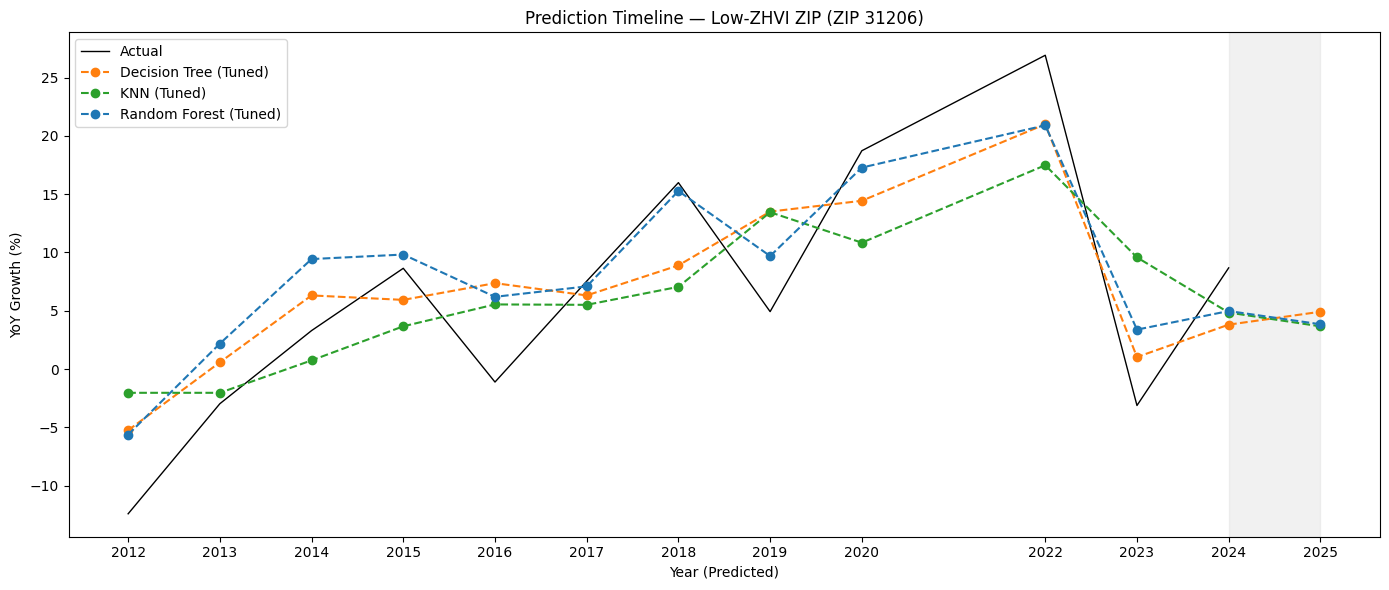
\includegraphics[width=\textwidth]{figures/timelineLow.png}
    \caption{Prediction trends over time for low-ZHVI ZIP}
    \caption*{\hspace{1em}}
    \label{fig:timeline_low}
\end{figure}
\FloatBarrier

\begin{figure}[!ht]
    \centering
    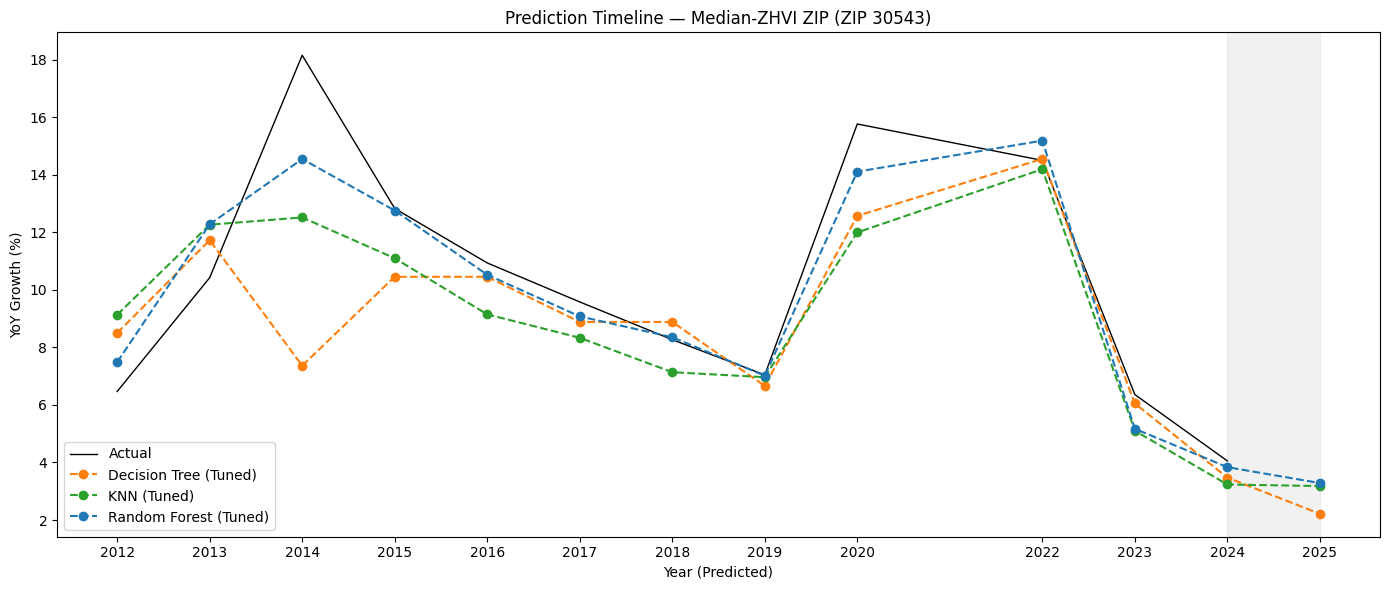
\includegraphics[width=\textwidth]{figures/timelineMedian.png}
    \caption{Prediction trends over time for median-ZHVI ZIP}
    \caption*{\hspace{1em}}
    \label{fig:timeline_median}
\end{figure}
\FloatBarrier

\begin{figure}[!ht]
    \centering
    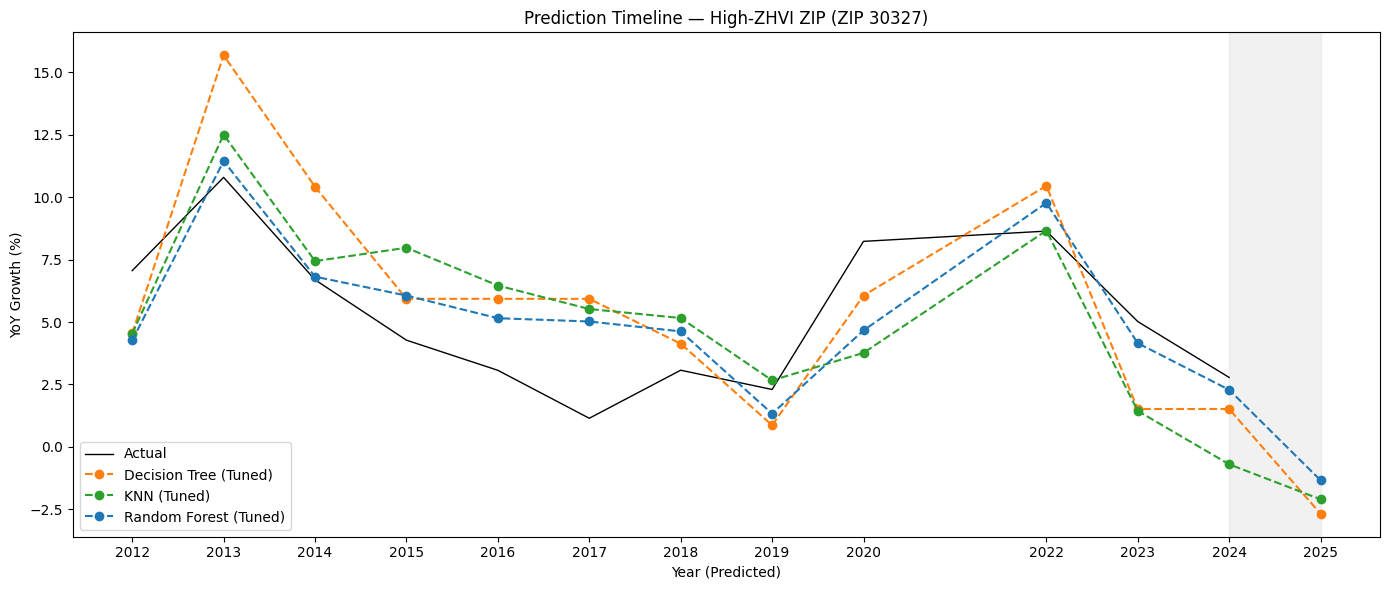
\includegraphics[width=\textwidth]{figures/timelineHigh.png}
    \caption{Prediction trends over time for high-ZHVI ZIP}
    \caption*{\hspace{1em}}
    \label{fig:timeline_high}
\end{figure}
\FloatBarrier

Across all three ZIP codes, the Random Forest model most consistently follows the actual YoY growth trend, particularly during years with noticeable dips or inflection points (e.g., 2016, 2019, 2023). In contrast, Decision Tree often smooths over or delays these changes, while KNN tends to flatten predictions and underestimates high-variance years. All models converge in the forecast period (2024–2025), but Random Forest shows closer alignment with the actual data in years prior, especially during periods of volatility.

\section{Summary}

All three models learned meaningful patterns from the data, but Random Forest consistently performed the best. It generalizes well across ZIPs, tracks yearly growth over time, and balances fit without overfitting. KNN was competitive, especially in areas with stable trends, but struggled with rapid market shifts. Decision Tree was the weakest, showing overfitting in training and poor generalization in both time and accuracy-based evaluations.
